% Start here


\chapter{Introduction}
\label{sec:intro}


The aim of this document is to report the results of the task T7.1 of WP7 :  "Primary tool Chain analyses and recommendations".


\section{T7.1 objective}

The objectives of this task are to identify the modelling languages, the tools and the tool platform suitable to define the primary tool chain of OpenETCS project. This primary tool chain shall  cover all specification and design activities of the OpenETCS process (part in blue in \ref{fig:main_process}). For more details see D2.3 \citep{D2_3} and D2.6-9 \citep{D2_6}. Means and tools for other activities described on figure \ref{fig:main_process} (mainly verification, validation and safety activities)  are going to be discussed during the task T7.2 of WP7.


 \begin{figure}
  \centering
  \fbox{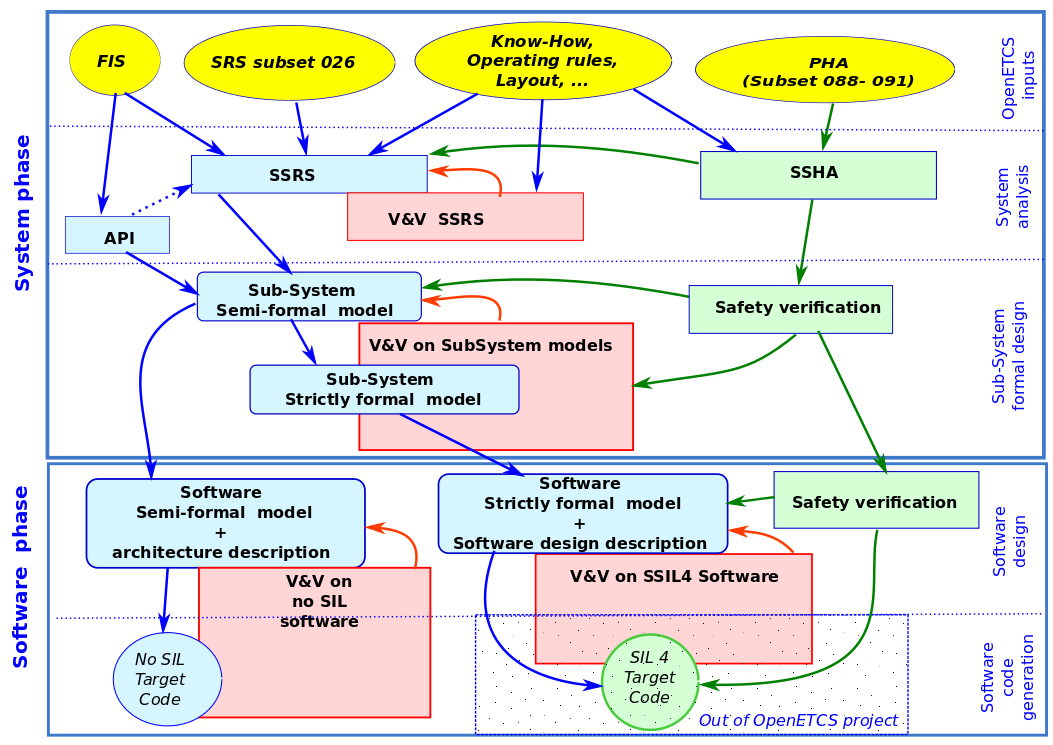
\includegraphics[scale=0.45]{images/WholeProcess.png}}
  \caption{Main OpenETCS process}
  \label{fig:main_process}
\end{figure}

\section{T7.1 activities}

The activities have started in November 2012, with a proposal of benchmark organisation.
After selection of a set of case studies (specified in D2.5 \citep{D2_5}), different approaches have been proposed and models have been stored on a common open github repository.
All the methods have been presented during a public meeting in April 2013.

Besides,  a set of criteria have been defined according the D2.6-9 requirement document \citep{D2_6}.  The results are recorded in the outputs O7.1.3-O7.1.7 \citep{WP7_O713_O717} for means and tools and O7.1.9 \citep{WP7_O719} for tool platform.

A decision meeting took place the 4th of July 2013 to analyse the results of the benchmark and to decide which means and tools will be retained during the process.

Results of the decision are given in this current document. 



%%%%%%%%%%%%%%%%%%%%%%%%%%%%%%%%%%%%%%%%%%%%%%%%%%%%%%%%%%%%%%%

\section{Glossary}
\label{sec:glossary}

\begin{description}
\item[API] Application Programming Interface
\item[FIS] Functional Interface Specification
\item[HW] Hardware
\item[I/O] Input/Output
\item[OBU] On-Board Unit
\item[PHA] Preliminary Hazard Analysis
\item[SIL] Safety Integrity Level
\item[SRS] System Requirement Specification
\item[SSHA] Sub-System Hazard Analysis
\item[SSRS] Sub-System Requirement Specification
\item[SW] Software
\item[V\&V] Verification \& Validation
\end{description}

%%%%%%%%%%%%%%%%%%%%%%%%%%%%%%%%%%%%%%%%%%%%%%%%%%%%%%%%%%%%%%%


